\documentclass[times, utf8, zavrsni, numeric]{fer}
\usepackage{booktabs}
\usepackage{graphicx}
\usepackage{amsmath}
\usepackage{physics}
\usepackage{ctable}
\usepackage{multirow}
\usepackage{algorithm}
\usepackage{algorithmic}
\graphicspath{ {./images/} }

\floatname{algorithm}{Algoritam}
\renewcommand{\algorithmiccomment}[1]{\bgroup\hfill//~#1\egroup}


\begin{document}

\thesisnumber{4830}
\title{Genetski algoritam inspiriran kvantnom mehanikom}
\author{Juraj Fulir}

\maketitle

% Ispis stranice s napomenom o umetanju izvornika rada. Uklonite naredbu \izvornik ako želite izbaciti tu stranicu.
\izvornik

\zahvala{
  
Zahvaljujem mentoru prof. dr. sc. Domagoju Jakoboviću na nesebičnoj pomoći, poticaju i savjetima u razvoju rada te danoj mogućnosti odabira vlastite teme. 
\\

Posebno zahvaljujem svojoj obitelji na podršci, razumijevanju i ljubavi tijekom školovanja te strpljenju tijekom kasnih noćnih sati. 
\\

Najtoplije zahvaljujem Karlu Kneževiću, mag. ing., te ostalim prijateljima, kolegicama i kolegama na korisnim savjetima i pomoći tijekom izrade završnog rada.
}

\tableofcontents

\chapter{Uvod}
Genetski algoritmi postoje još od 1960-tih kada je John Holland sa svojim studentima i kolegama napravio algoritam koji je simulirao fenomen adaptivnog ponašanja u prirodi. Kasnije su otkrivene mogućnosti i primjene genetskih algoritama na širokom rasponu stvarnih problema iz područja inženjerstva, ekonomije, kemije, robotike i mnogih drugih. Danas su genetski algoritmi podgrupa široke klase evolucijskih algoritama koji simuliranom evolucijom pronalaze rješenja. \citep{c_history}

\paragraph{}
U ovom se radu ostvaruje implementacija novije vrste genetskog algoritma koja za predstavljanje i manipuliranje podacima koristi paradigmu kvantne mehanike. Praktični dio implementiran je u sklopu evolucijskog razvojnog okruženja ECF (\it Evolutionary Computation Framework\rm) razvijenog na FER-u. U implementaciji se koristi aproksimacija qubita koja nije pronađena u ostalim radovima i člancima, a koja je isplativija u pogledu memorijskog zauzeća i kompleksnosti implementacije. Algoritam je prilagođen korištenju 3 različite reprezentacije genotipa: niz bitova, niz decimalnih brojeva i bitovni niz s pretvorbom u niz decimalnih brojeva. Vrši se usporedba algoritma s klasičnim genetskim algoritmom na tri različita problema, svaki za jednu reprezentaciju genotipa. Radu se prilažu svi rezultati te korišteni parametri. 

\paragraph{}
Rad je raspoređen na sljedeći način: u poglavlju \ref{ch:kvameh} ukratko se navodi povijest i opisuje značaj kvantne mehanike, objašnjavaju neki temeljni pojmovi potrebni za shvaćanje paradigme računanja kvantnim računalima te trenutna tržišna scena istih. U poglavlju \ref{ch:gaiqm} opisuje se struktura klasičnog genetskog algoritma i kvantnog genetskog algoritma te detaljnije genetski algoritam inspiriran kvantnom mehanikom. U poglavlju \ref{ch:primjena} opisuju se i prikazuju rezultati eksperimenata postignuti algoritmima CGA i GAIQM. 
%Uz to obavlja se i usporedba s ostalim postojećim algoritmima na problemu traženja minimuma funkcija. 
U poglavlju \ref{ch:nadogradnja} predlažu se moguće izmjene i nadogradnje algoritma. U dodatku \ref{ch:parametri} prilaže se popis svih podržanih parametara za komponente GAIQM.

\chapter{Kvantna mehanika i kvantna računala}
\label{ch:kvameh}
Do početka 19. stoljeća fizičari su imali deterministički pogled na svijet. Razvojem tehnologije koja je omogućavala promatranje sve manjih čestica primjećuju se fenomeni koje dotadašnja fizika nije mogla opisati. Iz potrebe za objašnjavanjem tih neobjašnjivih pojava razvijene su vrlo neintuitivne teorije koje, iako su matematički dokazane, nisu olako prihvaćene na znanstvenoj sceni. Jedna takva teorija je pretpostavka diskretne prirode stvarnosti. Iz nje je nastalo jedno čitavo područje fizike zvano \it kvantna mehanika\rm . Iako su puno ranije postojala slična razmišljanja o diskretnim i točkastim česticama (Arhimed, Demokrit, Galilei, Bošković), do 19. stoljeća nije postojala ni tehnologija kojom bi se tvrdnje dokazale ni matematika kojom bi se te tvrdnje opisale. Početkom 19. stoljeća, Max Planck objavljuje "\it Plankov zakon zračenja\rm" kojim rješava dugogodišnji problem opisivanja zračenja crnog tijela, popularno nazvan "\it ultraljubičasta katastrofa\rm". Definira povezanost izračene energije s valnom duljinom izračene svjetlosti, ali još bitnije definira diskretizirano zračenje u paketićima energije koje naziva 'količina', latinski 'kvantum'. Njegovim otkrićem kreće revolucija u fizici od kojih ću spomenuti samo nekoliko: otkriće fotoelektričnog efekta (Einstein), ispravljanje (redefiniranje) modela atoma (Rutherford, Bohr), otkriće dvojne prirode čestica (De Broglie), opisivanje valne prirode elektronske ljuske atoma (Heisenberg, Schr\"odinger, Born). \citep{bozja_cestica} Danas je kvantni pogled na svijet vrlo uvriježen u krugu fizičara i šire, no još nije u potpunosti shvaćen. Unatoč tome korištenjem fenomena proizišlih iz kvantne fizike stvorili smo razne uređaje i alate koji su danas u širokoj primjeni. Neki takvi uređaji su: tunel dioda, laser, magnetska rezonancija i drugi.

\paragraph{}
Ukratko, kvantna mehanika je relativno mlada grana fizike, ali je uvelike utjecala na razvoj tehnologije, znanosti i shvaćanja svijeta u kojem živimo.

\section{Temeljni pojmovi kvantne mehanike}

\subsection{Kvantna superpozicija}
Jedan je od osnovnih i nama najvažnijih pojmova kvantne mehanike.
Kvantna superpozicija je princip koji definira zbroj (superpoziciju) dvaju ili više kvantnih stanja kao ispravno kvantno stanje. 
To znači da je kvantno stanje kombinacija više stanja s pridijeljenom vrijednosti (važnosti) svakog stanja.

\paragraph{}
Kvantnom superpozicijom deterministički je model atoma s definiranim dozvoljenim putanjama elektrona zamijenjen puno preciznijim kvantnim modelom atoma koji ne definira točne putanje elektrona već prostornu distribuciju vjerojatnosti pronalaženja elektrona u određenoj točki prostora. Slikovito možemo reći da je model atoma s kružnim putanjama elektrona oko jezgre zamijenjen modelom jezgre okružene elektronskim oblacima. \citep{bozja_cestica}

\paragraph{}
Jedan od najpoznatijih alegorija superpozicije je Schr\"odingerov misaoni eksperiment zvan 'Schr\"odingerova mačka'. Zamislimo zatvorenu čeličnu kutiju u koju smo stavili mačku i Geigerov brojač unutar kojeg se nalazi uređaj s otrovom. Uređaj u sebi ima komadić radioaktivnog elementa, toliko malen da se u vremenskom rasponu od 1 sat može (ali i ne mora) dogoditi raspad atoma. U slučaju raspada Geigerov bojač aktivira relej koji ispusti čekić na malenu staklenu ampulu cijanovodične kiseline.
Ostavimo li sustav zatvorenim na sat vremena možemo reći da je mačka još uvijek živa ako u međuvremenu nije došlo do raspada atoma jer prvi bi raspad otrovao mačku. Psi (valna) funkcija čitavog sustava bi to opisala stanjima žive i mrtve mačke jednakog značaja, odnosno drugačije rečeno jednakih vjerojatnosti pojavljivanja.
Stvarno stanje ne možemo znati s potpunom sigurnošću dok ne otvorimo kutiju i pogledamo u nju.

\paragraph{}
Iz primjera vidimo da se sustav (ili čestica) može nalaziti u superpoziciji dok god ne promotrimo (izmjerimo) sustav. Superpozicija je opisana valnom funkcijom, a mjerenjem sustava gubi se superpozicija odnosno događa se kolaps valne funkcije u jedno determinističko stanje. Dakle, mjerenjem sustava dobivamo klasično stanje čestice u kojem se ona tog trena našla i upravo to je naša poveznica između "kvantnog" i "klasičnog" svijeta koja je nužna za ostvarivanje upotrebljivog kvantnog računala.

\subsection{Kvantna dekoherencija}
Kvantna dekoherencija je kolaps valne funkcije odnosno nepovratni gubitak pohranjene informacije zbog utjecaja okoline koja ga okružuje.
U stvarnim kvantnim sustavima relativno je lako ostvariti superpoziciju, ali je veliki problem održati ju. Ovisno o tehnologiji sustava razni uvjeti moraju biti ostvareni kako bi se sustav izolirao od okoline i zaštitio integritet pohranjene informacije. Iz tog su razloga kvantni sustavi danas glomazni i zahtjevni za održavanje.

\subsection{Spregnuta stanja}
Spregnuta kvantna stanja  \engl{entangled quantum states} povezana su (spregnuta) ako rezultat mjerenja jednog kvantnog stanja utječe na rezultat mjerenja drugog kvantnog stanja. Zanimljivost te veze je da se "informacija" o rezultatu mjerenja jednog stanja u istom trenu prenese drugom stanju. Poznati paradoks koji opisuje tu pojavu je "Einstein–Podolsky–Rosen paradoks".

\subsection{Teorem o nekloniranju}
Teorem o nekloniranju \engl{no-cloning theorem} jedna je velika zapreka u kvantnoj fizici. 
Njime se potvrđuje da nije moguće stvoriti identične kopije postojećeg kvantnog stanja. Želimo li stvoriti još jednu česticu nalik ovoj koju već imamo, moramo ponoviti čitav proces stvaranja te čestice. \cite{q_history}

\paragraph{}
Iako teorem djeluje vrlo ograničavajuće može se upotrijebiti u kvantnoj kriptografiji. Problem sigurnosti razmjene javnog ključa na kojoj se zasniva moderna sigurnost Interneta može se riješiti kvantnom enkripcijom kojom se garantira nemogućnost kopiranja odaslanog ključa. Čitanjem ključa uništava se njegovo kvantno stanje te ga nije moguće kopirati čime se ostvaruje zaštita od "\it Man-in-the-middle\rm" napada. \citep{han_phd}

\clearpage

\section{Kvantni bit (qubit)}
Kvantni bit je najmanja jedinica podatka u kvantnim računalima. U literaturi se može pronaći i pod nazivima "\it qbit\rm" i "\it Qbit\rm". Fizički gledano to je zapravo sićušna čestica sa svojstvom superpozicije.

\subsection{Princip rada}
\paragraph{}
Klasični bit pronalazimo u jednom od dva klasična stanja. Jednom postavljeno stanje se pamti i uvijek ga u njemu možemo pronaći. Njima gradimo binarni brojevni sustav pomoću kojeg zapisujemo podatke na računalu.

\paragraph{}
Kvantni bit ne pamti jedno klasično stanje već se on istovremeno nalazi u više različitih klasičnih stanja. To se svojstvo naziva superpozicija. Fizički gledano kvantni bit je čestica kojoj je pridružen kvantizirani spin. Spin je kvantizirana inačica kutne količine gibanja rotirajućeg tijela.

\paragraph{}
Kvantno stanje jednog qubita opisano je vektorom njegovog spina. Kvantno stanje opisuje vjerojatnost pronalaženja qubita u svakom od klasičnih stanja. Konkretno stanje dobivamo mjerenjem qubita kojim se uništava njegovo svojstvo superpozicije te dobivamo česticu u jednom stanju koju možemo koristiti poput klasičnog bita.

\begin{center}
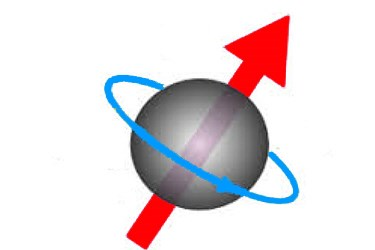
\includegraphics[width=55mm, height=40mm]{spin}
\captionof{figure}{Spin u obliku vektora na osi rotacije čestice.}
\end{center}

\paragraph{}
Sustavi s kvantnim bitovima mogu biti definirani za proizvoljan brojevni sustav, no s obzirom na to da su današnja računala bazirana na binarnom brojevnom sustavu zanima nas definicija qubita s 2 stanja.

\newpage

\subsection{Blochova sfera}
\paragraph{}
Stanje qubita prikazujemo Blochovom sferom. Jedno kvantno stanje prikazujemo kao vektor iz središta sfere na njenu površinu. Stanja u kojima možemo pronaći qubit prikazujemo polovima sfere koje definiramo sjecištima sfere i z-osi. \citep{computer_scientist}\citep{qubit_geometry}

\begin{center}
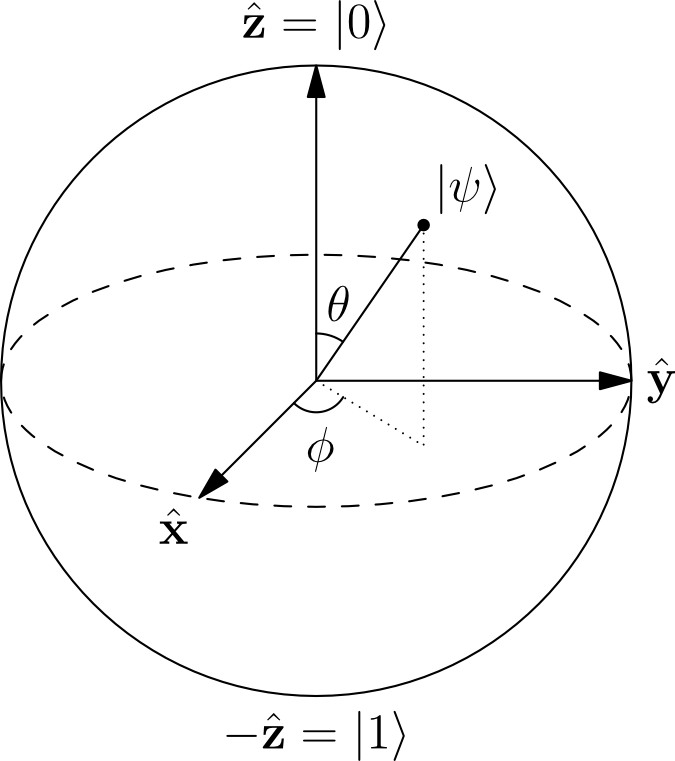
\includegraphics[width=60mm, height=65mm]{bloch}
\captionof{figure}{Blochova sfera}
\end{center}

\paragraph{}
Na slici vidimo jedno kvantno stanje opisano vektorom. Matematički ga možemo opisati kao linearnu kombinaciju dvaju klasičnih stanja:
\begin{align}
\ket{\psi} &= \alpha\ket{0} + \beta\ket{1} \label{eq:psi_orig}
\end{align}
gdje su $\alpha$ i $\beta$ kompleksni brojevi.

\paragraph{}
Iz vektora na Blochovoj sferi definiramo konstante iz \eqref{eq:psi_orig}:
\begin{align} \label{eq:psi_orig_full}
\ket{\psi} &= \cos(\frac{\theta}{2})\ket{0} + e^{i\phi}\cdot\sin(\frac{\theta}{2})\ket{1} \nonumber \\
&= \cos(\frac{\theta}{2})\ket{0} + (cos(\phi)+i\sin(\phi))\cdot\sin(\frac{\theta}{2})\ket{1} 
\end{align}

\paragraph{}
Vrijednosti $\alpha$ i $\beta$ su normirane:
\begin{equation} \label{eq:prob_norm}
|\alpha|^2 + |\beta|^2 = 1
\end{equation}

\paragraph{}
Vrijednosti $\alpha$ i $\beta$ predstavljaju vjerojatnosne amplitude pronalaženja qubita u stanju $\ket{0}$ i $\ket{1}$ respektivno.
Iz vjerojatnosnih amplituda računamo vjerojatnosti pronalaženja qubita u svakom od stanja:
\begin{equation} \label{eq:prob}
\begin{split}
\Pr{\ket{0}} = |\alpha|^2 = \cos^2{\frac{\theta}{2}} \\ 
\Pr{\ket{1}} = |\beta|^2 = \sin^2{\frac{\theta}{2}}
\end{split}
\end{equation}

\paragraph{}
Kvantno stanje možemo zapisati vektorom što je pogodno za izvršavanje matričnih operacija nad njime. \citep{computer_scientist}
\begin{align}
\ket{\psi} =
\begin{bmatrix}
\alpha \\ \beta
\end{bmatrix}
\end{align}

\subsection{Aproksimacija kvantnog stanja}
\paragraph{}
Kvantno stanje prikazano na Blochovoj sferi opisano je s 3 dimenzije. Trodimenzionalne operacije računski su vrlo zahtjevne stoga želimo pojednostaviti model kvantnog stanja. 
U simulaciji rada s qubitom jedino su nam važne vjerojatnosti pronalaženja qubita u određenom stanju. 
Iz formula \eqref{eq:prob_norm} i \eqref{eq:prob} zaključujemo da vjerojatnost $|\beta|^2$ ovisi isključivo o vjerojatnosti $|\alpha|^2$:
\begin{align*}
|\alpha|^2 + |\beta|^2 &= 1 \\
|\beta|^2 &= 1 - |\alpha|^2 \\
&= 1 - \cos^2\frac{\theta}{2} \\
&= \sin^2\frac{\theta}{2}
\end{align*}

Ako bolje pogledamo kvantno stanje opisano formulom \eqref{eq:psi_orig_full} vidjet ćemo da $\alpha$ ovisi samo o kutu $\theta$. Želimo se riješiti kompleksne konstante $\beta$ ili ju barem svesti na realnu.
Iz jednakosti \eqref{eq:phi_useless} zaključujemo da je kut $\phi$ suvišan za računanje vjerojatnosti. To možemo vidjeti i na samoj Blochovoj sferi.
Za fiksni kut $\theta$ mijenjanjem kuta $\phi$ rotiramo vektor oko z-osi i ne približavamo se niti jednom polu sfere odnosno vjerojatnosti stanja se ne mijenjaju.
\begin{equation}
\label{eq:phi_useless}
|cos(\phi)+i\sin(\phi)| = 1
\end{equation}

Dakle, parametre $\alpha$ i $\beta$ sveli smo na realne vrijednosti koje ovise samo o jednom parametru: $\theta$. Naše kvantno stanje možemo opisati formulom:
\begin{align} 
\label{eq:aprox_real}
\ket{\psi} = \cos(\frac{\theta}{2})\ket{0} + \sin(\frac{\theta}{2})\ket{1} 
\end{align}

\paragraph{}
Aproksimacijom qubita uz zadržane vjerojatnosti stanja dobivamo sljedeću reprezentaciju kvantnog stanja qubita:

\begin{center}
\includegraphics[width=80mm, height=72mm]{approx}
\captionof{figure}{Aproksimacija qubita}
\end{center}

\begin{align}
\label{eq:qubit_aprox}
\begin{split}
\alpha = \cos\frac{\theta}{2} \qquad
\beta = \sin\frac{\theta}{2}
\end{split}
\end{align}
\begin{equation}
\label{eq:qubit_state_aprox}
\ket{\psi} = \cos(\frac{\theta}{2})\ket{0} + \sin(\frac{\theta}{2})\ket{1}
\end{equation}

\subsection{Kvantni registar}
Kvantni registar, poput klasičnog registra, pohranjuje niz qubita te omogućuje ne-destruktivno čitanje i zapisivanje istih. Ovdje čitanje predstavlja korištenje (izmjena) kvantnog stanja zapisanog u njemu, a ne mjerenje koje bi uništilo superpoziciju qubita.
\begin{figure}[htb]
\centering
\begin{align*}
\begin{bmatrix}
q_1 & q_2 & q_3 & \cdots & q_i & \cdots & q_n
\end{bmatrix}
\end{align*}
\caption{Registar qubita}
\end{figure}

\newpage

Simulacija kvantnog registra koju implementiraju članci na koje sam naišao je klasični registar koji pohranjuje vjerojatnosne amplitude qubita pomoću kojih se određuju vjerojatnosti stanja. \citep{han_qga_combinat}\citep{han_analysis}\citep{han_phd}
\begin{figure}[htb]
\centering
\begin{align*}
\begin{bmatrix}
\alpha_1 & \alpha_2 & \alpha_3 & \cdots & \alpha_i & \cdots & \alpha_n \\
\beta_1 & \beta_2 & \beta_3 & \cdots & \beta_i & \cdots & \beta_n
\end{bmatrix}
\end{align*}
\caption{Registar aproksimiranih qubita zapisom gustoća vjerojatnosti}
\end{figure}

Koristeći aproksimaciju qubita zadanu formulom \ref{eq:qubit_state_aprox} zapis stanja možemo dodatno pojednostaviti tako da u klasični registar pohranjujemo samo kuteve qubita pomoću kojih možemo izračunati vjerojatnosti stanja.
\begin{figure}[htb]
\centering
\begin{align*}
\begin{bmatrix}
\theta_1 & \theta_2 & \theta_3 & \cdots & \theta_i & \cdots & \theta_n \\
\end{bmatrix}
\end{align*}
\caption{Registar aproksimiranih qubita zapisom kuteva kvantnog stanja}
\end{figure}

\paragraph{}
Za implementaciju je odabran posljednji navedeni model kvantnog registra zbog svoje jednostavnosti i memorijske isplativosti. Kasniji će se operatori također pojednostaviti zahvaljujući ovoj aproksimaciji.

\clearpage

\section{Kvantni algoritmi i kvantna računala}
Kvantno računalo je uređaj koji je sposoban izvršavati matematičke i logičke zadatke korištenjem fenomena kvantne mehanike. Temeljna podatkovna jedinica klasičnog računala je bit, a kvantnog računala qubit. Prednost qubita posjedovanje svojstva superpozicije kojim se otvara mogućnost pohrane više klasičnih stanja odjednom. Jedan primjer primjene qubita je kvantni registar kao spremnik podataka kojim se ističe značaj superpozicije:
\begin{quote}
Pomoću 1 klasičnog registra veličine n bitova moguće je pohraniti 1 od mogućih $2^n$ vrijednosti.

Pomoću 1 kvantnog registra veličine n qubita moguće je pohraniti $2^n$ od mogućih $2^n$ vrijednosti, odnosno sve vrijednosti odjednom. \citep{qga}
\end{quote}

\paragraph{}
Zanimanje za kvantnim računalima počinje rasti 1980-tih godina govorom Richarda Feynmana u kojem Feynman iznosi i obrazlaže zabrinutost da se kvantni sustavi ne mogu učinkovito simulirati klasičnim računalom, umjesto kojeg predlaže osnovni model kvantnog računala. \citep{q_history}\citep{feynman}

\paragraph{}
Kvantni algoritam je algoritam prilagođen elementima kvantnog računala. Kvantnim algoritmima moguće je ostvariti značajna ubrzanja nekih NP problema.\cite{qga_apply}\citep{han_phd} Primjeri takvih algoritama su:
\begin{itemize}
\item Shorov algoritam faktorizacije cijelih brojeva - moguća primjena u otkrivanju javnog ključa (RSA)
\item Groverov algoritam invertiranja funkcije - moguća primjena u pretraživanju baze podataka
\item Simulacije kvantnih sustava
\end{itemize}

\clearpage

\section{Trenutno stanje u svijetu}
Porastom snage i pouzdanosti kvantnih računala krenulo se stvarati tržište za njih. Danas neke od najvećih tvrtki ulažu u razvoj kvantnih računala. To su većinom banke, vojska i IT industrija.
Danas su najpoznatije dvije tvrtke koje proizvode i razvijaju kvantna računala.

\subsubsection{D-Wave}
Tvrtka D-Wave razvija i proizvodi kompaktne zatvorene sustave kvantnih računala. Trenutno najnoviji model kvantnog računala tvrtke D-Wave je 2000Q, podržava 2000 qubita i temelji se na adijabatskom kvantnom računanju. Rješava probleme pretraživanja prostora principom sličnim simuliranom kaljenju. Ta su računala nedostupna široj javnosti isključivo zbog svoje cijene (15 milijuna američkih dolara, 05.2017.) no neke su ih tvrtke ipak nabavile (Google, NASA, USRA, Volkswagen Group i ostali).

\subsubsection{IBM}
IBM nudi udaljeni pristup svojim kvantnim računalima koja su razvili. Javni paket uključuje pristup web aplikaciji za dizajniranje kvantnih krugova do 5 qubita te mogućnost izvršavanja eksperimenta na simulatoru ili stvarnom kvantnom procesoru. Pristup stvarnom kvantnom procesoru naplaćuje se 'virtualnim kreditom' koji se dobiva registracijom na sustav i vremenski obnavlja. Svako izvršavanje se naplaćuje ovisno o zadanom broju ponoavljanja eksperimenta. Početkom 2017. godine omogućen je pristup računalu s čak 20 qubita preko web aplikacije. Postoji API za razvoj kvantnih krugova pomoću "kvantnog asemblera" (QASM), a u tijeku je izrada API-a za pristup sustavu kojim bi se omogućio razvoj algoritama i aplikacija u više programskih jezika.

\chapter{Genetski algoritam inspiriran kvantnom mehanikom} 
\label{ch:gaiqm}
U ovom se odlomku opisuju sličnosti između klasičnog i kvantnog genetskog algoritma te primjena aproksimacije qubita u genetskom algoritmu inspiriranom kvantnom mehanikom. Posebno se opisuje rad GAIQM te njegova implementacija.

\paragraph{}
Svi navedeni algoritmi koriste i evaluator.
To je procedura koja jedinci pridružuje vrijednost dobrote \engl{fitness} prema kojoj se poželjnije jedinke ističu iz populacije. Gradi se ovisno o zadanom problemu i ne ovisi o implementaciji algoritma odnosno jednom napisani evaluator je kompatibilan sa svim algoritmima. Ovisi jedino o načinu na koji se zapisuju podaci koji se evoluiraju tj. ovisi o vrsti genotipa.

\section{Klasični genetski algoritam (CGA)}
\subsection{Dijelovi}
Klasični genetski algoritam zahtjeva nekoliko osnovnih dijelova:
\begin{itemize}
\item Genotip 
\item Operator križanja 
\item Operator mutacije
\end{itemize}

\subsubsection{Genotip}
Podatkovna struktura koja opisuje jednu jedinku. Mora biti kompatibilna s evaluatorom i zahtjeva sebi kompatibilne operatore. Sadrži kromosom u obliku niza bitova.
\begin{figure}[htb]
\centering
\begin{align*}
\begin{bmatrix}
b_1 & b_2 & b_3 & \cdots & b_i & \cdots & b_n
\end{bmatrix}
\end{align*}
\caption{Registar klasičnih bitova}
\end{figure}

\subsubsection{Operator križanja}
Operator koji izvodi križanje (razmjenu) genetskog materijala danih jedinki. Odabire se točka koja će podijeliti kromosom roditelja na 2 dijela. Stvaraju se djeca kojima je jedna polovica roditelja zamijenjena polovicom drugog roditelja.
\begin{figure}[htb]
\centering
\begin{align*}
Roditelj 1:
\begin{bmatrix}
\mathbf{b_{11}} & \mathbf{b_{12}} & | & b_{13} & \cdots & b_{1i} & \cdots & b_{1n}
\end{bmatrix} \\
Roditelj 2:
\begin{bmatrix}
\mathbf{b_{21}} & \mathbf{b_{22}} & | & b_{23} & \cdots & b_{2i} & \cdots & b_{2n}
\end{bmatrix} \\\\
Dijete 1:
\begin{bmatrix}
\mathbf{b_{21}} & \mathbf{b_{22}} & b_{13} & \cdots & b_{1i} & \cdots & b_{1n}
\end{bmatrix} \\
Dijete 2:
\begin{bmatrix}
\mathbf{b_{11}} & \mathbf{b_{12}} & b_{23} & \cdots & b_{2i} & \cdots & b_{2n}
\end{bmatrix}
\end{align*}
\caption{Križanje kromosoma zamjenom polovica roditeljskih kromosoma}
\end{figure}

\subsubsection{Operator mutacije}
Operator koji vrši izmjenu genetskog materijala dane jedinke. Odabire se bit koji se invertira.
\begin{figure}[htb]
\centering
\begin{align*}
\begin{bmatrix}
b_1 & b_2 & \mathbf{b_3} & \cdots & b_i & \cdots & b_n
\end{bmatrix}\\
\begin{bmatrix}
b_1 & b_2 & \overline{\mathbf{b_3}} & \cdots & b_i & \cdots & b_n
\end{bmatrix}
\end{align*}
\caption{Mutacija invertiranjem jednog bita kromosoma}
\end{figure}

\newpage

\subsection{Pseudokod}
U nastavku je dan pseudokod općenitog genetskog algoritma koji se izvršava na klasičnom računalu.
\begin{algorithm}
\caption{Klasični genetski algoritam (CGA)}
\label{algo:cga}
\begin{algorithmic}
\STATE{\textbf{Input:\ $parametri$}}
\STATE{$InicijalizirajPopulaciju\ $P(0)}
\STATE{$EvaluirajPopulaciju\ $P(0)}
\STATE{B = $DohvatiNajboljegIz\ $P(0)}
\WHILE{$NijeDovoljnoDobar\ $B}
\STATE{t $\gets$ t + 1}
\STATE{$OdaberiRoditeljeIz\ $P(t)}
\STATE{$OperatorKrizanja$}
\STATE{$OperatorMutacije$}
\STATE{$EvaluirajPopulaciju\ $P(t)}
\ENDWHILE
\RETURN $B$
\end{algorithmic}
\end{algorithm}

\newpage

\section{Kvantni genetski algoritam (QGA)}
\subsection{Dijelovi}
Kvantni genetski algoritam uz svoje specifične operatore sadrži i dijelove slične onima iz CGA:
\begin{itemize}
\item Kvantni genotip (kvantni registar)
\item Kvantna rotacijska vrata
\item Inicijalizator populacije
\item Operator mjerenja qubita
\end{itemize}

\subsubsection{Kvantni genotip (kvantni registar)}
Podatkovna struktura koja opisuje jednu jedinku. Od klasičnog registra se razlikuje u principu pohrane podataka (superpozicija). Zahtjeva operatore sposobne za baratanje qubitima. Dodatno zahtjeva i klasični genotip koji može pohraniti izmjerene vrijednosti qubita i koji je pogodan evaluatoru. Sadrži kromosom u obliku niza qubita.
\begin{figure}[htb]
\centering
\begin{align*}
\begin{bmatrix}
q_1 & q_2 & q_3 & \cdots & q_i & \cdots & q_n
\end{bmatrix}
\end{align*}
\caption{Registar qubita}
\end{figure}

\subsubsection{Operator kvantnih rotacijskih vrata}
Ovim se operatorom mijenja kvantno stanje qubita. Koristi se za unaprjeđenje populacije transformacijom kromosoma. Matematički se može prikazati kao matrica koja mora biti unitarna odnosno mora vrijediti: $UU^{\dagger} = I$.

\paragraph{}
Prisjetimo se da smo kvantno stanje qubita opisali vektorom na Blochovoj sferi. Želimo li promijeniti stanje qubita moramo rotirati svojstveni vektor. Upravo nam tome služe kvantna rotacijska vrata. Najvažnija vrata su vrata identiteta i Paulijeva X, Y i Z vrata:
\begin{equation}
I = 
\begin{bmatrix}
1 & 0 \\ 0 & 1
\end{bmatrix} \quad
X = 
\begin{bmatrix}
0 & 1 \\ 1 & 0
\end{bmatrix} \quad
Y = 
\begin{bmatrix}
0 & -i \\ i & 0
\end{bmatrix} \quad
Z = 
\begin{bmatrix}
1 & 0 \\ 0 & -1
\end{bmatrix}
\end{equation}

\paragraph{}
Matematički primjenu kvantnih rotacijskih vrata ostvarujemo umnoškom kvantnog stanja zapisanog u vektor i samih vrata, npr. ostvarenje zrcaljenja oko x-osi:
\begin{equation}
X\cdot \ket{\psi} = 
\begin{bmatrix}
0 & 1 \\ 1 & 0
\end{bmatrix} \cdot
\begin{bmatrix}
\alpha \\ \beta
\end{bmatrix}
= \begin{bmatrix}
\beta \\ \alpha
\end{bmatrix}
\end{equation}

\paragraph{}
Kvantna rotacijska vrata u QGA mogu poprimiti više namjena. U prethodnom primjeru zrcaljenjem oko x-osi zamjenjujemo vjerojatnosti pronalaska bita u oba stanja, odnosno ostvarujemo operaciju sličnu inverziji bita koja se koristi za mutaciju kromosoma. Manjom rotacijom kvantnog stanja oko x-osi ili y-osi približavamo se stanju $\ket{0}$ ili $\ket{1}$ te tako ostvarujemo pretraživanje prostora stanja.

\subsubsection{Inicijalizator populacije}
Svrha inicijalizatora populacije je postaviti qubite u superpoziciju. Ostvaruje se Hadamardovim H vratima:
\begin{equation}
H = \frac{1}{\sqrt{2}}
\begin{bmatrix}
1 & 1 \\ 1 & -1
\end{bmatrix} 
\end{equation}

\paragraph{}
Matematički prikaz postavljanja qubita u superpoziciju:
\begin{equation}
H\cdot \ket{\psi} = \frac{1}{\sqrt{2}}
\begin{bmatrix}
1 & 1 \\ 1 & -1
\end{bmatrix} \cdot
\begin{bmatrix}
\alpha \\ \beta
\end{bmatrix}
 = \frac{1}{\sqrt{2}}
\begin{bmatrix}
\alpha + \beta \\ \alpha - \beta
\end{bmatrix}
\end{equation}
Na samom početku qubit nije u superpoziciji te se može nalaziti u stanju $\ket{0}$ ili $\ket{1}$. Primjenom Hadamardovih vrata na takve qubite dobivamo dvije istovjetne superpozicije stanja.
\begin{align}
\begin{split}
H \cdot \ket{0} &= \frac{1}{\sqrt{2}}
\begin{bmatrix}
1 + 0 \\ 1 - 0
\end{bmatrix}
= \begin{bmatrix}
\frac{1}{\sqrt{2}} \\ \frac{1}{\sqrt{2}}
\end{bmatrix}
\\
H \cdot \ket{1} &= \frac{1}{\sqrt{2}}
\begin{bmatrix}
0 + 1 \\ 0 - 1
\end{bmatrix}
= \begin{bmatrix}
\frac{1}{\sqrt{2}} \\ -\frac{1}{\sqrt{2}}
\end{bmatrix}
\end{split}
\end{align}
Istovjetnost superpozicija zaključujemo iz formule \ref{eq:prob} kojom dobivamo jednake vjerojatnosti za oba stanja.
\begin{equation}
|\alpha|^2 = |\beta|^2 = \frac{1}{2}
\end{equation}

\subsubsection{Operator mjerenja qubita}
Operator mjerenja qubita uništava kvantnu superpoziciju qubita i pretvara ju u klasično determinističko stanje, odnosno pretvara qubit u bit. Kvantnim stanjem qubita opisana je vjerojatnost pronalaženja qubita u jednom klasičnom stanju.

\subsection{Pseudokod}
U nastavku je dan pseudokod kvantnog genetskog algoritma koji se izvršava na kvantnom računalu, izuzev evaluacije koja je prilagođena i izvršava se klasičnom računalu.

\begin{algorithm}
\caption{Kvantni genetski algoritam (QGA)}
\label{algo:qga}
\begin{algorithmic}
\STATE{\textbf{Input:\ $parametri$}}
\STATE{$InicijalizirajPopulaciju\ $Q(0)}
\STATE{$OperatorMjerenja\ $Q(0) $\to$ P(0)}
\STATE{$EvaluirajPopulaciju\ $P(0)}
\STATE{B = $DohvatiNajboljegIz\ $P(0)}
\WHILE{$NijeDovoljnoDobar\ $B}
\STATE{t $\gets$ t + 1}
\STATE{$OperatorKvantnihRotacijskihVrata\ $Q(t)}
\STATE{$OperatorMjerenja\ $Q(t) $\to$ P(t)}
\STATE{$EvaluirajPopulaciju\ $P(t)}
\STATE{B = $DohvatiNajboljegIz\ $P(t)}
\ENDWHILE
\RETURN $B$
\end{algorithmic}
\end{algorithm}

\newpage

\section{Genetski algoritam inspiriran kvantnom mehanikom (GAIQM)}
Genetski algoritam inspiriran kvantnom mehanikom je simulacija QGA. U literaturi ga možemo pronaći i pod nazivom "\it Quantum inspired genetic algorithm (QIGA)\rm". \citep{han_phd}

\subsection{Dijelovi}
GAIQM sadrži dijelove CGA i QGA prilagođene korištenoj aproksimaciji qubita:
\begin{itemize}
\item Kvantni genotip (kvantni registar)
\item Operator kvantnih rotacijskih vrata
\item Kvantni operator mutacije
\item Operator katastrofe
\item Inicijalizator populacije
\item Operator mjerenja qubita
\end{itemize}

\subsubsection{Kvantni genotip (kvantni registar)}
Podatkovna struktura koja opisuje jednu jedinku. Od stvarnog kvantnog registra se razlikuje u principu pohrane podataka. Superpozicija qubita zapisana je aproksimacijom kvantnog stanja qubita (formula \ref{eq:qubit_state_aprox}) tj. kutem kvantnog stanja.
\begin{figure}[htb]
\centering
\begin{align*}
\begin{bmatrix}
\theta_1 & \theta_2 & \theta_3 & \cdots & \theta_i & \cdots & \theta_n
\end{bmatrix}
\end{align*}
\caption{Registar kuteva aproksimiranog kvantnog stanja qubita}
\end{figure}

\subsubsection{Operator kvantnih rotacijskih vrata}
Rotaciju qubita proizvoljnim kutem $\delta\theta$ u dvodimenzionalnom prostoru ostvarujemo rotacijskim vratima:
\begin{align}
\begin{bmatrix}
\alpha' \\ \beta'
\end{bmatrix}
=
\begin{bmatrix}
\cos(\delta\theta) & -\sin(\delta\theta) \\ \sin(\delta\theta) & \cos(\delta\theta)
\end{bmatrix}
\begin{bmatrix}
\alpha \\ \beta
\end{bmatrix}
\end{align} 

\paragraph{}
Koristeći aproksimaciju qubita zadanu formulom \ref{eq:qubit_state_aprox} operator rotacije možemo pojednostaviti:
\begin{align*}
\begin{bmatrix}
\alpha' \\ \beta'
\end{bmatrix}
&=
\begin{bmatrix}
\cos(\delta\theta) & -\sin(\delta\theta) \\ \sin(\delta\theta) & \cos(\delta\theta)
\end{bmatrix}
\begin{bmatrix}
\alpha \\ \beta
\end{bmatrix}
\\&=
\begin{bmatrix}
\cos(\delta\theta) & -\sin(\delta\theta) \\ \sin(\delta\theta) & \cos(\delta\theta)
\end{bmatrix}
\begin{bmatrix}
\cos(\frac{\theta}{2}) \\ \sin(\frac{\theta}{2})
\end{bmatrix}
\\&=
\begin{bmatrix}
\cos(\frac{\theta}{2})\cos(\delta\theta) - \sin(\frac{\theta}{2})\sin(\delta\theta) \\ \cos(\frac{\theta}{2})\sin(\delta\theta) + \sin(\frac{\theta}{2})\cos(\delta\theta)
\end{bmatrix}
\\&=
\begin{bmatrix}
\cos(\frac{\theta}{2}+\delta\theta) \\ \sin(\frac{\theta}{2}+\delta\theta)
\end{bmatrix} 
\\
\begin{bmatrix}
\cos(\frac{\theta'}{2}) \\ \sin(\frac{\theta'}{2})
\end{bmatrix}
&=
\begin{bmatrix}
\cos(\frac{\theta+2\delta\theta}{2}) \\ \sin(\frac{\theta+2\delta\theta}{2})
\end{bmatrix}
\end{align*}

\paragraph{}
Zaključujemo da je matrično množenje moguće zamijeniti formulom znatno manje složenosti:
\begin{align} \label{eq:qrot_simple}
\theta' = \theta + 2\cdot \delta\theta
\end{align}

\paragraph{}
Kut zakreta $\delta\theta$ je moguće zadati pomoću tablice kuteva tzv. \it look-up table\rm\ u kojoj za svaki mogući slučaj određujemo smjer i veličinu zakreta. Tablicu možemo proizvoljno zadati, a standardni oblik tablice dan je u nastavku:
\begin{table}[htb]
\caption{Standardna \it look-up\rm\ tablica}
\label{tbl:lookup}
\centering
\begin{tabular}{|c|c|c|c|c|c|c|c|} 
\hline
$q_i$ & $b_i$ & f(q)>f(b) & $\Delta\theta$ & \multicolumn{4}{|c|}{sg($\alpha_i, \beta_i$)} \\
\hline
&&&& $\alpha_i\cdot\beta_i$ > 0 & $\alpha_i\cdot\beta_i$ < 0 & $\alpha_i$ = 0 & $\beta_i$ = 0 \\
\hline
0 & 0 & $\bot$ & 0 & - & - & - & - \\
0 & 0 & $\top$ & 0 & - & - & - & - \\
0 & 1 & $\bot$ & $\phi$ & +1 & -1 & 0 & $\pm$1 \\
0 & 1 & $\top$ & $\phi$ & -1 & +1 & $\pm$1 & 0 \\
1 & 0 & $\bot$ & $\phi$ & -1 & +1 & $\pm$1 & 0 \\
1 & 0 & $\top$ & $\phi$ & +1 & -1 & 0 & $\pm$1 \\
1 & 1 & $\bot$ & 0 & - & - & - & - \\
1 & 1 & $\top$ & 0 & - & - & - & - \\
\hline
\end{tabular}
\end{table}
\paragraph{}
Za zadani i-ti qubit neke jedinke $q$ i i-ti qubit najbolje jedinke $b$, ovisno o odnosu vrijednosti dobrote jedinki odabiremo redak u tablici.
Kut zakreta čitamo iz retka na sljedeći način:
\begin{align*}
\delta\theta = \Delta\theta \cdot sg(a,b)
\end{align*}
gdje $\Delta\theta$ određuje iznos zakreta, a $sg(\alpha_i, \beta_i)$ smjer zakreta. Vrijednost kut $\phi$ se najčešće odabire iz intervala $[0.005\pi, 0.01\pi]$.

\paragraph{}
U praksi se pokazalo da male promjene vrijednosti zadanih tablicom uvelike utječu na brzinu i pouzdanost čitavog algoritma. Ovim pristupom određivanja kuta moguće je ostvariti prilagodbu algoritma pojedinom problemu i ostvariti dobre rezultate, no ugađanje konstanti nije učinkovito zbog njihove brojnosti, ima ih čak 40. Stvara se i problem fiksne vrijednosti zakreta zbog koje dolazi do prebrze konvergencije populacije čime ona gubi raznolikost i često završava u lokalnom optimumu. Prevelik kut zakreta sprječava finu pretragu oko pronađenog optimuma što ograničava preciznost pretrage.

\paragraph{}
Iz tih se razloga koristi adaptivno ugađanje vrijednosti zakreta koje automatski prilagođava iznos kuta zakreta.\citep{adaptive_qga} Umjesto fiksne vrijednosti kuta $\phi$ zadajemo najveću i najmanju vrijednost kuta između kojih će se interpolirati vrijednost kuta $\phi$. Što je jedinka bliža najboljoj jedinci po vrijednosti dobrote, to je kut zakreta manji, odnosno kut zakreta proporcionalan je razlici vrijednosti dobrota jedinki. Formula za određivanje kuta je sljedeća:

\begin{equation}
\label{eq:adapt}
\delta\theta = l + (h - l) \cdot \frac{f(q) - f(w)}{f(b) - f(w))}
\end{equation}
gdje $l$ i $h$ predstavljaju respektivno iznos donje i gornje granice kuta zakreta, $f(q)$ vrijednost funkcije dobrote za jedinku koju usmjeravamo, a $f(b)$ i $f(w)$ vrijednost funkcije dobrote za respektivno najbolju i najgoru jedinku u trenutnoj populaciji. Ovom je formulom omogućen valjan odabir kuta zakreta istovremeno za probleme minimizacije i maksimizacije.

\newpage

\subsubsection{Kvantni operator mutacije}
Koriste se dvije vrste mutacija koje se izvršavaju ili ne ovisno o zadanoj vjerojatnosti izvršavanja: inverzija i zamjena.

\paragraph{}
Operator inverzije nasumično određuje jedan qubit jedinke te ga invertira. Mutacija je izvedena po uzoru na onu iz QGA. Obavlja se zrcaljenje bita s obzirom na x-os. Aproksimacijom stanja qubita samo jednim kutem (\ref{eq:qubit_aprox}) ograničili smo kut $\theta$ na interval $[-\pi, \pi]$ te omogućili pojednostavljeno zrcaljenje kuta:
\begin{algorithm}
\caption{Kvantni operator mutacije za GAIQM}
\label{algo:gaiqm_mut}
\begin{algorithmic}
\STATE{\textbf{Input:\ $\theta$}}
\IF{$\theta$ > 0}
\RETURN $\pi - \theta$
\ELSE
\RETURN $-\pi - \theta$
\ENDIF
\end{algorithmic}
\end{algorithm}

\paragraph{}
Operator zamjene nasumično odabire dva qubita te im zamjenjuje mjesta.
\begin{figure}[htb]
\centering
\begin{align*}
\begin{split}
\begin{bmatrix}
\boldsymbol{\theta_{1}} & \theta_{2} & \boldsymbol{\theta_{3}} & \cdots & \theta_{i} & \cdots & \theta_{n}
\end{bmatrix} 
\\
\begin{bmatrix}
\boldsymbol{\theta_{3}} & \theta_{2} & \boldsymbol{\theta_{1}} & \cdots & \theta_{i} & \cdots & \theta_{n}
\end{bmatrix}
\end{split}
\end{align*}
\caption{Zamjena dva nasumično odabrana qubita}
\label{fig:mut_swap}
\end{figure}

\subsubsection{Operator katastrofe}
Uporabom operatora kvantnih rotacijskih vrata algoritam može konvergirati u lokalni optimum, koji nije globalni optimum, te u njemu zaglaviti. Same mutacije nisu dovoljne da bi se algoritam izvukao, već je potreban snažniji operator.

\paragraph{}
Operator katastrofe unosi velik poremećaj u populaciju čime ostvaruje veću raznolikost populacije, a time i pretraživanje šireg prostora stanja. Operator sve jedinke populacije izuzev najbolje, vraća u početno stanje superpozicije. Te jedinke tada ponovno konvergiraju ("iz nule"), ali ovog puta odmah kreću prema pronađenoj najboljoj jedinci. Iako se najbolja jedinka nalazi u lokalnom optimumu, nasumično stvorene jedinke započinju svoju konvergenciju iz više različitih stanja povećavajući vjerojatnost pretraživanja dosad neistraženog prostora.

\paragraph{}
Prečestim pozivanjem operatora može se blokirati svojstvo usmjerenog razvoja populacije čime se pretraživanje pretvara u nasumično. To reguliramo parametrom ponovljenih optimuma. Ideja je pratiti u koliko se uzastopnih generacija ponavlja ista vrijednost najbolje jedinke, a kada taj broj prekorači vrijednost parametra izvršavamo katastrofu.
\begin{algorithm}
\caption{Okidač katastrofe}
\label{algo:katastrofa_okidac}
\begin{algorithmic}
\STATE{\textbf{Input:\ }B} \COMMENT{\it Vrijednost dobrote najbolje jedinke u populaciji.\rm}
\IF{$prekoracen(parametarOkidanja)$} 
\STATE{$resetirajBrojac()$}
\RETURN{true}
\ELSIF{$najboljiSePonovio(B)$}
\STATE{$uvecajBrojac()$}
\ELSE
\STATE{$resetirajBrojac()$}
\STATE{$zapamtiNajboljeg(B)$}
\ENDIF
\RETURN{false}
\end{algorithmic}
\end{algorithm}

\subsubsection{Inicijalizator populacije}
Inicijalizator postavlja sve qubite u stanje superpozicije $\ket{\psi_0}$.
%\begin{align*}
%\alpha = \cos{\frac{\theta}{2}} \qquad \beta = \sin{\frac{\theta}{2}} \\
%\ket{\psi_0} = H \cdot \ket{\psi} &= \frac{1}{\sqrt{2}}
%\begin{bmatrix}
%\alpha + \beta \\ \alpha - \beta
%\end{bmatrix}
%\\ &=
%\begin{cases}
%\frac{1}{\sqrt{2}} \alpha \ket{0} + \frac{1}{\sqrt{2}} \beta \ket{1} \\
%\frac{1}{\sqrt{2}} \alpha \ket{0} - \frac{1}{\sqrt{2}} \beta \ket{1}
%\end{cases}
%\\ &=
%\begin{cases}
%\frac{1}{\sqrt{2}} \cos{\frac{\theta}{2}} \ket{0} + \frac{1}{\sqrt{2}} \sin{\frac{\theta}{2}} \ket{1} \\
%\frac{1}{\sqrt{2}} \cos{\frac{\theta}{2}} \ket{0} - \frac{1}{\sqrt{2}} \sin{\frac{\theta}{2}} \ket{1}
%\end{cases}
%\end{align*}
 Zbog aproksimacije qubita definirane formulom \ref{eq:qubit_state_aprox} potrebno je sve kuteve inicijalizirati na $\pm\frac{\pi}{2}$.
%\begin{align*}
%\ket{\psi_0} = \begin{cases}
%\frac{1}{2} \ket{0} + \frac{1}{\sqrt{2}} \sin{\frac{\theta}{2}} \ket{1} \\
%\frac{1}{\sqrt{2}} \cos{\frac{\theta}{2}} \ket{0} - \frac{1}{\sqrt{2}} \sin{\frac{\theta}{2}} \ket{6}
%\end{cases}
%\end{align*}
 
\subsubsection{Operator mjerenja}
Operatorom mjerenja superpoziciju pretvaramo u klasično stanje odnosno qubit pretvaramo u bit. Koje će stanje poprimiti pojedini qubit ovisi o njegovom kvantnom stanju prema formuli za izračun vjerojatnosti (\ref{eq:prob}).
\begin{algorithm}
\caption{Operator mjerenja}
\label{algo:op_mjerenja}
\begin{algorithmic}
\STATE{\textbf{Input:\ }$\theta_i$} \COMMENT{\it Kut kvantnog stanja i-tog qubita.\rm}
\IF{$nasumicanBroj(0,1) > \cos^2(\theta_i / 2)$} 
\RETURN{1}
\ELSE
\RETURN{0}
\ENDIF
\end{algorithmic}
\end{algorithm}

\newpage

\subsection{Pseudokod}
U nastavku je dan pseudokod genetskog algoritma inspiriranog kvantnom mehanikom koji se izvršava na klasičnom računalu.

\begin{algorithm}
\caption{Genetski algoritam inspiriran kvantnom mehanikom (GAIQM)}
\label{algo:gaiqm}
\begin{algorithmic}
\STATE{\textbf{Input:\ $parametri$}}
\STATE{$InicijalizirajPopulaciju\ $Q(0)}
\STATE{$OperatorMjerenja\ $Q(0) $\to$ P(0)}
\STATE{$EvaluirajPopulaciju\ $P(0)}
\STATE{B = $DohvatiNajboljegIz\ $Q(0), P(0)}
\WHILE{$NijeDovoljnoDobar\ $B}
\STATE{t $\gets$ t + 1}
\IF{$OkidacKatastrofe\ $B}
\STATE{$OperatorKatastrofe\ $B, Q(t)}
\ENDIF
\STATE{$OperatorKvantnihRotacijskihVrata\ $B, Q(t)}
\STATE{$OperatorMutacije\ $Q(t)}
\STATE{$OperatorMjerenja\ $Q(t) $\to$ P(t)}
\STATE{$EvaluirajPopulaciju\ $P(t)}
\STATE{B = $DohvatiNajboljegIz\ $Q(t), P(t)}
\ENDWHILE
\RETURN $B$
\end{algorithmic}
\end{algorithm}

\newpage

\section{Implementacija algoritma}
Algoritam je implementiran korištenjem aproksimacije qubita i kvantnog registra.
\subsubsection{Kvantni genotip (QuantumRegister)}
Genotip nasljeđuje klasu Binary koja svoj kromosom zapisuje u obliku niza bitova, a nudi i pretvorbu niza bitova u niz realnih brojeva. Definiranim parametrima \ref{tbl:param_kvareg} određuje se brojnost i preciznost pretvorenih realnih brojeva. Dodatno sadrži i registar koji pamti samo vrijednosti kuteva aproksimiranih kvantnih stanja.
\begin{figure}[htb]
\centering
\begin{align*}
Registar\ bitova &
\begin{bmatrix}
b_1 & b_2 & b_3 & \cdots & b_i & \cdots & b_n \\
\end{bmatrix} \\
Registar\ realnih\ brojeva &
\begin{bmatrix}
r_1 & r_2 & r_3 & \cdots & r_j & \cdots & r_m \\
\end{bmatrix} \\
Registar\ kuteva &
\begin{bmatrix}
\theta_1 & \theta_2 & \theta_3 & \cdots & \theta_i & \cdots & \theta_n \\
\end{bmatrix}
\end{align*}
\caption{$QuantumRegister$ sadrži 3 registra za reprezentaciju informacije}
\end{figure}

\paragraph{}
Sadrži metodu $measure()$ kojom se izvršava mjerenje registra. Iteracijom po kutevima računa se vjerojatnost i određuje klasično stanje (bit) koje se zapisuje u registar bitova. Algoritam koji određuje stanje qubita:
\begin{algorithm}
\caption{measure()}
\label{algo:measure}
\begin{algorithmic}
\FOR{$\theta _i$ : registarKuteva}
\STATE{$b _i$ = randomDouble() > $\cos^2{(\frac{\theta _i}{2})}$}
\ENDFOR
\end{algorithmic}
\end{algorithm}

\paragraph{}
Metodom $resetQubits(StateP)$ ostvaruje se inicijalizacija superpozicije qubita. Parametrima \ref{tbl:param_kvareg} moguće je odrediti kut početne superpozicije. Ova metoda nasumično postavlja pozitivan ili negativan početni kut za svaki qubit, te nakon toga poziva $measure()$ kako bi se iz qubita dobile vrijednosti bitova. Konačno poziva se metoda $update()$ naslijeđena iz klase $Binary$ koja pretvara binarni zapis registra bitova u realne vrijednosti ovisno o zadanim granicama i preciznosti realnih vrijednosti. Ova se metoda poziva i pri inicijalizaciji samog kvantnog registra.

\paragraph{Napomena:}
Nasljeđujući $Binary$ genotip sadrži sve potrebne podatkovne strukture i procedure klase $Binary$ te se može jednako koristiti. To znači da evaluatori koji koriste $Binary$ mogu direktno koristiti i $QuantumRegister$ bez potrebe za dodatnim (pomoćnim) genotipom što za taj slučaj ubrzava rad algoritma.

\subsubsection{GAIQM}
Implementacija GAIQM prati pseudokod \ref{algo:gaiqm}. Algoritam interno koristi $QuantumRegister$ nad kojim izvršava sve potrebne operacije. Kako bi algoritam podržavao različite genotipe kompatibilne s više evaluatora dodan je i prilagodnik \engl{adapter}.

\paragraph{}
Prilagodnik u obliku metode $adapter(individual, indexOfQreg)$ kopira odgovarajući sadržaj kvantnog registra u radni genotip koji se koristi u evaluatoru. Ovisno o tipu kopira samo realne brojeve ($FloatingPoint$) ili samo bitove ($BitString$ i $Binary$). Posebno se za $Binary$ nakon kopiranja poziva metoda $update()$ kako bi se osvježili i realni brojevi tog genotipa. Metoda se neće pozvati ako je $QuantumRegister$ jedini zadani genotip. Jedinka može imati više genotipa koji su pohranjeni u niz, a varijabla $indexOfQreg$ služi kao indeks na kojem se nalazi genotip kvantnog registra. 

\paragraph{Napomena:}
Algoritam se služi konvencijom da je $QuantumRegister$ uvijek posljednji genotip u jedinki. Zato treba paziti da se pri definiciji parametara genotipa $QuantumRegister$ uvijek navede posljednji.

\subsubsection{MutQuantumInversion}
Operator inverzije pri pozivu nasumično odabire jedan qubit u zadanom registru te ga invertira algoritmom \ref{algo:gaiqm_mut}.

\subsubsection{MutQuantumSwap}
Operator zamjene pri pozivu nasumično odabire dvije različite pozicije qubita u zadanom registru te im zamjeni vrijednosti kao što je prikazano slikom \ref{fig:mut_swap}.

\subsubsection{QuantumRotationGate}
Koristi se pojednostavljena formula \ref{eq:qrot_simple} i adaptivna metoda izračuna vrijednosti zakreta \ref{eq:adapt}. Tablica predznaka je implementirana neizravno pomoću $if-else$ blokova.

\chapter{Eksperimenti} 
\label{ch:primjena}
Eksperiment se sastoji od usporedbe CGA i GAIQM na identičnom eksperimentu uz parametre za koje pojedini algoritam ostvaruje dobre rezultate.
Terminator eksperimenata je maksimalan broj evaluacija koji je zadan ovisno o problemu koji rješava.
Svaki eksperiment je ponovljen 40 puta, a prikazani rezultati su usrednjene vrijednosti ponovljenih eksperimenata.

\section{Problem naprtnjače}
\subsection{Opis problema}
Zadana je nosivost naprtnjače \engl{knapsack} i popis predmeta. Za svaki predmet zadana je njegova težina i vrijednost.
Cilj je pronaći najvrjedniju kombinaciju stvari uz uvjet da nije prekoračena nosivost naprtnjače.
Dobrota jedinke računa se sumom vrijednosti svih odabranih predmeta.
Ovaj eksperiment koristi genotip $BitString$.

\subsection{Rezultati}
Za testiranje koristim nasumično generirani skup predmeta s ograničenom maksimalnom težinom predmeta, maksimalnom vrijednošću predmeta te definiranim brojem predmeta u setu. Koristim skupove od 500 i 1000 predmeta. Statistike skupova i parametri algoritma dani su u nastavku.

\begin{table}[htb]
\caption{Statistike skupova predmeta}
\centering
\begin{tabular}{r>{\centering\arraybackslash}p{2.5cm}>{\centering\arraybackslash}p{2.5cm}} \hline
Značajka & Skup 500 & Skup 1000 \\ 
\hline
Veličina naprtnjače & 100 & 100 \\
Broj predmeta & 500 & 1000 \\
Najveća vrijednost & 100 & 100 \\
Najveća težina & 70 & 100 \\
Najmanja težina & 1 & 1 \\
Prosječna težina & 36.598 & 51.365 \\
Optimalna vrijednost & 2922 & 3616 \\
\hline
\end{tabular}
\end{table}

\paragraph{}
\begin{table}[htb]
\caption{Korišteni parametri za problem naprtnjače}
\centering
\begin{tabular}{|l|c||l|c|} \hline
\multicolumn{2}{|c||}{SteadyStateTournament} & \multicolumn{2}{c|}{GAIQM} \\ 
\hline
Parametar & Vrijednost & Parametar & Vrijednost \\ 
\hline
tsize & 3 & disaster & 500 \\
&& qrot.ubound & 0.2 \\
&& qrot.lbound & 0.005 \\
&& initAngle & 0.01 \\
population.size & 100 & population.size & 10 \\
mutation.indprob & 0.3 & mutation.indprob & 0.04 \\
crx.onepoint & 1 & mut.quantum\_swap & 1 \\
mut.simple & 1 & mut.quantum\_inversion & 1 \\
\hline
\end{tabular}
\end{table}

\newpage

\paragraph{}
Pri evaluaciji rješenja može doći do pretrpavanja naprtnjače. Ne prihvaćamo takva rješenja te ih želimo potisnuti. To obavlja operator kazne ugrađen u evaluator koji ovisno o veličini prekoračenja umanjuje ostvareni profit za količinu prekoračene težine pomnoženu sa zadanom konstantom. Koristi se pretpostavljena konstanta $5$.

\newpage

\begin{table}[htb]
\caption{Prosječni rezultati po skupovima}
\centering
\begin{tabular}{|c|ccc|} \hline
\multirow{2}{*}{Skup} & \multicolumn{3}{c|}{CGA} \\ \cline{2-4}
 & Prosječno najbolje rješenje & Broj generacija & Broj evaluacija \\ 
\hline
500 & 2922 & 539 & 108030 \\
1000 & 3616 & 696 & 139405 \\
\hline
\end{tabular}
\end{table}
\begin{table}[htb]
\centering
\begin{tabular}{|c|ccc|} \hline
\multirow{2}{*}{Skup} & \multicolumn{3}{c|}{GAIQM} \\ \cline{2-4}
 & Prosječno najbolje rješenje & Broj generacija & Broj evaluacija \\ 
\hline
500 & 2922 & 3088 & 30909 \\
1000 & 3616 & 4215 & 42175 \\
\hline
\end{tabular}
\end{table}
\paragraph{}
Oba algoritma za oba seta pronalaze optimalno rješenje. Ovdje je posebno naglašena razlika u broju poziva evaluatora. Vidimo da je za set od 1000 predmeta GAIQM 3 puta manje poziva evaluator.
\begin{center}
\includegraphics[width=60mm, height=70mm]{Knapsack500} \hspace{15mm}
\includegraphics[width=60mm, height=70mm]{Knapsack1000}
\captionof{figure}{Odnos algoritama na setovima veličine 500 i 1000 predmeta}
\end{center}

\subsection{Utjecaj parametara}
GAIQM ima više parametara u odnosu na CGA te zahtjeva više konfiguracije. Iako sama implementacija ima pretpostavljenu većinu parametara, ovisno o problemu potrebno je uštimati pojedine parametre kako bi se ostvarili bolji rezultati. Navedeni primjeri i mjerenja definirani su za prethodno izmjereni skup od 500 predmeta.

\subsubsection{Veličina populacije}
Većom populacijom ostvaruje se veća raznolikost genetskog materijala što pospješuje pretraživanje neistraženog prostora stanja što znači da će algoritam u manje generacija pronaći optimalno rješenje. Što je veća populacija, to će se po generaciji više puta pozivati evaluator koji je često vrlo zahtjevan i spor. Dakle, želimo pronaći optimalnu veličinu populacije za koju će se minimizirati broj poziva evaluatora.

\begin{table}[htb]
\caption{Prosječan broj evaluacija i generacija ovisno o veličini populacije}
\centering
\begin{tabular}{rrr} \hline
Veličina populacije & Broj evaluacija & Broj generacija \\ 
\hline
3 &	35496 &	11830.1 \\
10	 & 33542 &	3352.2 \\
30 &	35127 &	1168,9 \\
50	 & 45200 &	902.0 \\
100 &	73990 &	737.9 \\
\hline
\end{tabular}
\end{table}
\begin{center}
\includegraphics[width=140mm, height=80mm]{populacija}
\captionof{figure}{Broj evaluacija za zadanu veličinu populacije}
\end{center}

Za sve navedene veličine populacija algoritam pronalazi optimalno rješenje. Vidimo da broj evaluacija ovisi o veličini populacije te da za ovaj konkretan problem ima minimum za populaciju 10 jedinki. S druge strane, broj generacija opada porastom veličine populacije što potvrđuje tvrdnju o značaju raznolikosti populacije.

\subsubsection{Početni kut}
Početnim kutom definiramo stanje u kojem će se pronaći svi qubiti pri inicijalizaciji. Standardno se postavlja na $\frac{\pi}{2}$ no može se mijenjati ovisno o problemu. Za problem naprtnjače ovisno o karakteristikama skupa koji koristimo možemo pretpostaviti da će većina ili manjina predmeta stati u naprtnjaču. Tada početni kut postavljamo na veći ili manji kut respektivno.

\begin{table}[htb]
\caption{Prosječan broj evaluacija i generacija ovisno o početnom kutu}
\centering
\begin{tabular}{rrr} \hline
Početni kut & Broj evaluacija & Broj generacija \\ 
\hline
0.005 &	51443	& 5142.3 \\
0.01 & 	33542 & 	3352.2 \\
0.05 &	 91165 & 	9114.5 \\
0.1 &	78141 &	7812.1 \\
0.5 &	200000 &	19998.0 \\
0.7 &	200000 &	19998.0 \\
\hline
\end{tabular}
\end{table}

\begin{center}
\includegraphics[width=140mm, height=80mm]{kutevi}
\captionof{figure}{Broj evaluacija za zadani početni kut qubita}
\end{center}

\paragraph{}
Vidimo da naša pretpostavka o svojstvima skupa može uvelike utjecati na brzinu, ali i uspješnost rada algoritma. Pri odabiru ponovno postoje optimalni parametri za koje algoritam postiže najveću brzinu. Na ovom primjeru algoritam za početne kuteve $0.5 \pi$ i $0.7 \pi$ ne pronalazi rješenje već se prekida brojem evaluacija dok za kut $0.1 \pi$ gotovo uvijek pronalazi rješenje problema.

\subsubsection{Granice kuteva adaptivne metode zakreta}
Granice kuteva su vrlo osjetljivi parametri izrazito ovisni o problemu. Adaptivnom metodom odabir kuta zakreta bira se kao interpolacija vrijednosti unutar granica proporcionalno odnosu vrijednosti dobrote jedinke s najboljom jedinkom. Donja granica određuje preciznost kojom se pretražuju stanja oko najbolje jedinke trenutne populacije i obično je reda veličine $10^{-2}$ ili manje.  Gornja granica određuje početnu brzinu konvergencije kada jedinka ima najlošiju vrijednost dobrote u odnosu na najbolju vrijednost trenutne populacije i obično je reda veličine $10^{-1}$ ili manje. 

\paragraph{}
Kada algoritam pronađe lokalni optimum sve jedinke konvergiraju prema njoj. Dakle, premala donja granica može zaglaviti algoritam u lokalnom optimumu te se odabire vrijednost veća od 0. Prevelika gornja granica može uzrokovati prebrzu početnu konvergenciju populacije prema pronađenom lokalnom optimumu u kojem algoritam može zaglaviti. Raspon granica kuteva određuje brzinu konvergencije populacije te se često odabiru granice različite za 1 red veličine.

\subsubsection{Operator katastrofe}
Operator katastrofe poziva se samo kada se ista vrijednost dobrote pojavi u $n$ uzastopnih generacija. Bez njega algoritam može zapeti u lokalnom optimumu. Pozivamo li operator prečesto možemo usporiti ili čak zaustaviti konvergenciju populacije te algoritam neće moći pronaći optimum u razumnom vremenu. Operator treba pozivati "dovoljno" rijetko, a taj iznos ovisi o problemu i najbolje ga je odabrati prateći ponašanje rezultata tijekom rada algoritma. Uobičajene vrijednosti su reda 100 generacija.

\clearpage

\section{Traženje globalnog minimuma funkcije}
\subsection{Opis problema}
Zadane su netrivijalne višedimenzionalne funkcije kojima je potrebno pronaći minimum.
Ovaj eksperiment koristi genotip $FloatingPoint$ za klasični algoritam te $QuantumRegister$ kao radni genotip.

\paragraph{}
Zadane funkcije:
\begin{enumerate}
\item Kvadratna
\begin{equation}
f(\mathbf {x} )=\sum _{{i=1}}^{n}(x_{i}-i)^{2}
\end{equation}
\item Schaffer-ova F6 funkcija
\begin{equation}
f(x,y)=0.5+\frac{sin^2(\sqrt{x^2 + y^2})-0.5}{[1+0.001 \cdot (x^2 + y^2)]^2}
\end{equation}
\item Griewangk
\begin{equation}
f(x_1 \cdots x_n) = 1 + \frac{1}{4000} \sum_{i=1}^n x^2_i - \prod_{i=1}^n cos(\frac{x_i}{\sqrt{i}})
\end{equation}
\item Ackley
\begin{equation}
f(x_0 \cdots x_n) = -20 exp(-0.2 \sqrt{\frac{1}{n} \sum_{i=1}^n x_i^2}) - exp(\frac{1}{n} \sum_{i=1}^n cos(2\pi x_i)) + 20 + e
\end{equation}
\item Rastrigin
\begin{equation}
f(x_1 \cdots x_n) = 10n + \sum_{i=1}^n (x_i^2 -10cos(2\pi x_i))
\end{equation}
\item Rosenbrock
\begin{equation}
f(x_1 \cdots x_n) = \sum_{i=1}^{n-1} (100(x_i^2 - x_{i+1})^2 + (1-x_i)^2)
\end{equation}
\item Schaffer-ova F7 funkcija
\begin{equation}
f(x_0 \cdots x_n) = [\frac{1}{n-1}\sqrt{s_i} \cdot (sin(50.0s_i^{\frac{1}{5}})+1)]^2 s_i = \sqrt{x_i^2 + x_{i+1}^2}
\end{equation}
\end{enumerate}

\subsection{Rezultati}
Funkcije ograničavamo na 20 dimenzija/vrijednosti te prostor pretraživanja definiramo na intervalu $[-10, 10]$ preciznošću do 16. decimale.

\begin{table}[htb]
\caption{Korišteni parametri za $FunctionMin$}
\centering
\begin{tabular}{|l|c||l|c|} \hline
\multicolumn{2}{|c||}{SteadyStateTournament} & \multicolumn{2}{c|}{GAIQM} \\ 
\hline
Parametar & Vrijednost & Parametar & Vrijednost \\ 
\hline
tsize & 3 & disaster & 300 \\
&& qrot.ubound & 0.25 \\
&& qrot.lbound & 0.008 \\
&& initAngle & 0.5 \\
dimension & 20 & dimension & 20 \\
ubound & 10 & ubound & 10 \\
lbound & -10 & lbound & -10 \\
&& precision & 16 \\
population.size & 100 & population.size & 10 \\
mutation.indprob & 0.3 & mutation.indprob & 0.04 \\
&& mut.quantum\_swap & 0.2 \\
&& mut.quantum\_inversion & 0.8 \\
\hline
\end{tabular}
\end{table}

\paragraph{}
Za svaki eksperiment postavljena je granica dozvoljenog broja evaluacija na $200000$ te vrijednost maksimalne dozvoljene greške na $10^{-9}$. Algoritmi nikada ne dostižu vrijednosti globalnog optimuma pa je broj evaluacija jedini prekidač programa.

\clearpage

\paragraph{}
\begin{table}[htb]
\caption{Prosječne vrijednosti po funkcijama}
\centering
\begin{tabular}{|l|>{\centering\arraybackslash}p{2.5cm}|>{\centering\arraybackslash}p{2.5cm}|} \hline
\multirow{2}{*}{Funkcija} & \multicolumn{2}{c|}{Prosječno odstupanje} \\ \cline{2-3}
& CGA & GAIQM \\
\hline
F1 & $385$ & $387.65$ \\
F2 & $3.93\cdot 10^{-2}$ & $8.22\cdot 10^{-2}$ \\
F3 & $2.1\cdot 10^{-3}$ & $2.17\cdot 10^{-2}$ \\
F4 & $7.37\cdot 10^{-4}$ & $4.33\cdot 10^{-5}$ \\
F5 & $5.42\cdot 10^{-4}$ & $25.72$ \\
F6 & $26.36$ & $76$ \\
F7 & $1.92$ & $2.1$ \\
\hline
\end{tabular}
\end{table}

\paragraph{}
Za isti broj evaluacija GAIQM prolazi više generacija od CGA. Unatoč tome GAIQM ne pronalazi uvijek bolja rješenja. Dapače, ponekad pronalazi i po nekoliko redova veličine lošija rješenja.

\section{Regresija neuronske mreže}
\subsection{Opis problema}
Za zadane ulaz/izlaz brojčane podatke potrebno je pronaći težine veza između slojeva neuronske mreže (učenje neuronske mreže). Dobrota mreže računa se srednjom kvadratnom greškom (MSE) koju algoritam pokušava minimizirati. Ovaj eksperiment koristi genotip $FloatingPoint$.

\paragraph{}
Za testiranje koristim dvije funkcije:
\begin{align*}
&f(x) = \frac{x^2}{100},\quad x \in [-9, 9], \quad \Delta x = 1 \\
&g(x) = \sin{x},\quad x \in [0, 6.2], \quad \Delta x = 0.1
\end{align*}

\newpage

\subsection{Rezultati}
Struktura mreže je fiksirana na $1\to 5\to 1$, a aktivacijske funkcije su definirane po slojevima $sigmoidalna \to linearna$. Za svaki eksperiment postavljena je granica dozvoljenog broja evaluacija na $200000$ te vrijednost maksimalne dozvoljene greške na $10^{-9}$. Algoritmi nikada ne dostižu vrijednosti globalnog optimuma pa je broj evaluacija jedini prekidač programa.

\begin{table}[htb]
\caption{Korišteni parametri za regresiju neuronske mreže}
\centering
\begin{tabular}{|l|c||l|c|} \hline
\multicolumn{2}{|c||}{SteadyStateTournament} & \multicolumn{2}{c|}{GAIQM} \\ 
\hline
Parametar & Vrijednost & Parametar & Vrijednost \\ 
\hline
tsize & 3 & disaster & 600 \\
&& qrot.ubound & 0.1 \\
&& qrot.lbound & 0.01 \\
&& initAngle & 0.5 \\
population.size & 70 & population.size & 10 \\
mutation.indprob & 0.3 & mutation.indprob & 0.01 \\
&& mut.quantum\_swap & 1 \\
&& mut.quantum\_inversion & 1 \\
\hline
\end{tabular}
\end{table}

\paragraph{}
Težine između slojeva ograničavamo na interval $[-10, 10]$ s preciznošću do 16. decimale.

\paragraph{}
\begin{table}[htb]
\caption{Prosječni rezultati po funkcijama}
\centering
\begin{tabular}{|p{2.5cm}|>{\centering\arraybackslash}p{2.5cm}|>{\centering\arraybackslash}p{2.5cm}|} \hline
\multirow{2}{*}{Funkcija} & \multicolumn{2}{c|}{Prosječna greška} \\ \cline{2-3}
& CGA & GAIQM \\
\hline
$f(x)$ & $8.14\cdot 10^{-2}$ & $2.07\cdot 10^{-1}$ \\
$g(x)$ & $26.14$ & $26.36$ \\
\hline
\end{tabular}
\end{table}

\paragraph{}
GAIQM postiže znatno lošije rezultate u odnosu na CGA. Tijekom rada algoritam ne uspijeva izaći iz lokalnog optimuma te se operator katastrofe redovito poziva pokušavajući pronaći "bolji put" kojim će pretraživati prostor približavajući se optimumu.

%\section{COCO}
%\subsection{Opis problema}
%Algoritam se uspoređuje s ostalim algoritmima implementiranim u ECFu na problemu traženja minimuma funkcije ($FunctionMin$).
%
%\subsection{Rezultat}
%\begin{table}[htb]
%\caption{Korišteni parametri za COCO}
%\centering
%\begin{tabular}{|c|c|} \hline
%\multicolumn{2}{|c|}{GAIQM} \\ 
%\hline
%Parametar & Vrijednost \\ 
%\hline
%disaster & 500 \\
%qrot.ubound & 0.2 \\
%qrot.lbound & 0.005 \\
%initAngle & 0.01 \\
%population.size & 10 \\
%mutation.indprob & 0.04 \\
%mut.quantum\_swap & 1 \\
%mut.quantum\_inversion & 1 \\
%\hline
%\end{tabular}
%\end{table}
%
%GRAFOVI

\chapter{Moguće nadogradnje} \label{ch:nadogradnja}
\section{Paralelizacija}
Stvaranjem više nezavisnih populacija jedinki te povremenom razmjenom najboljih jedinki populacija poboljšava se raznolikost populacije. Također, ostvaruje se šira pretraga prostora stanja jer se jedinke pojedinih populacija počinju "kretati" prema drugim optimumima čime se povećava vjerojatnost pronalaženja dotad neistraženih stanja. \citep{han_phd}

\section{Podržavanje više-genotipskih jedinki}
Trenutno je ostvarena podrška jedinki s jednim genotipom. Definiranjem više genotipa, vrijednosti iz kvantnog registra će se kopirati u prvi zadani genotip (genotip jedinke na indeksu 0). Podršku više genotipa moguće je ostvariti izmjenom 'prilagodnika' \engl{adapter} te prikladnim zastavicama za odabir genotipova u koje će se kopirati odgovarajuće vrijednosti iz kvantnog registra.

\section{Ubrzanje algoritma domenom cijelih brojeva}
Operacije s podacima dvostruke preciznosti su računski zahtjevnije cjelobrojnih te ih je poželjno zamijeniti. Trenutno se u kvantni registar pohranjuju brojevi dvostruke preciznosti te su sve operacije prilagođene njihovom. Kako je kvantni i klasični dio GAIQM međusobno izoliran, a povezan samo operatorom mjerenja, moguće je drugačije modelirati kvantni dio bez utjecaja na klasični.

\paragraph{}
Umjesto decimalnih brojeva, u kvantni registar možemo pohranjivati cijele brojeve. Trenutnu definiciju kuta iz domene $[-\pi, \pi]$ možemo preslikati na proizvoljnu cjelobrojnu domenu $[MIN, MAX]$. Tada se sve operacije nad kvantnim registrom trebaju prilagoditi novoj domeni.

\paragraph{}
Nedostatak ove optimizacije je smanjivanje domene kuteva odnosno kvantnih stanja što može utjecati na preciznost lokalne pretrage prostora stanja kao i uzrokovati prebrzu konvergenciju stanja prema lokalnom optimumu.

\chapter{Zaključak} 
\label{ch:zaključak}
Genetski algoritam inspiriran kvantnom mehanikom kombinacija je strukture klasičnih genetskih algoritama i paradigme kvantnih računala. Cilj ovog rada je objasniti paradigmu kvantnih računala, istražiti mogućnosti oblikovanja stohastičkih optimizacijskih algoritama uz korištenje simulacije rada kvantnog računala te usporediti novu vrstu genetskog algoritma s klasičnim na nekoliko primjera.

\paragraph{}
Kako su evaluatori često skupe (spore) procedure, a brzina algoritma ovisi direktno o broju evaluacija poželjno je što manje pozivati evaluator. Rezultati usporedbe klasičnog genetskog algoritma (CGA) i genetskog algoritma inspiriranog kvantnom mehanikom (GAIQM) pokazuju na nadmoć GAIQM po broju poziva evaluatora. To navodi na činjenicu da je GAIQM iznimno pogodan za rad sa zahtjevnim evaluatorima. 

\paragraph{}
Vremenska cijena GAIQM proizlazi iz činjenice da obavlja računske operacije koje se ponavljaju nad svakim qubitom svake jedinke u populaciji. Svoju vremensku zahtjevnost balansira znatno manjom populacijom od CGA. Veličina populacije osigurava veću raznolikost populacije odnosno pretraživanje većeg prostora stanja po iteraciji te se na nju oslanja CGA. GAIQM s druge strane ne zahtijeva veliku populaciju zbog svoje ugrađene nasumičnosti svake jedinke kojom jednako dobro pretražuje prostor stanja.

\paragraph{}
Rezultati eksperimenata ukazuju na nadmoć GAIQM u kombinatoričkom tipu problema, konkretno na problemu naprtnjače. Na ostalim izvedenim eksperimentima GAIQM daje loše rezultate i ne uspijeva se mjeriti s CGA.

\bibliographystyle{fer}
\bibliography{literatura}

\appendix
\chapter{Parametri} 
\label{ch:parametri}
U nastavku je dan opis svih parametara. Obavezni parametri označeni su \textbf{podebljanim tekstom}.

\begin{table}[htb]
\caption{Parametri za <GAIQM>}
\label{tbl:param_gaiqm}
\centering
\begin{tabular}{p{2cm}ccp{8cm}} \hline
Naziv & Tip & Pretp. vr. & Opis\\ \toprule
$ubound$ & $double$ & 0.1 & Gornja granica zakreta qubita \\
$lbound$ & $double$ & 0.01 & Donja granica zakreta qubita \\
$disaster$ & $uint$ & -1 & Broj ponovljenih vrijednosti operatora katastrofe (vrijednost -1 gasi operator katastrofe) \\ \bottomrule
\end{tabular}
\end{table}

\begin{table}[htb]
\caption{Parametri za <KnapsackEvalOp>}
\label{tbl:param_knapsack}
\centering
\caption*{\footnotesize Parametri $dimension$, $ubound$, $lbound$ i $precision$ naslijeđeni su iz genotipa Binary.}
\begin{tabular}{p{4cm}ccp{6cm}} \hline
Naziv & Tip & Pretp. vr. & Opis\\ \toprule
$\textbf{eval.knapsackSize}$ & $double$ & - & Veličina (nosivost) torbe \\
$\textbf{eval.itemsFile}$ & $string$ & - & Putanja do datoteke s definicijama težina i cijene predmeta \\
$eval.$ $punishmentFactor$ & $double$ & 5 & Faktor kojim se množi prekoračenje nosivosti torbe \\ \bottomrule
\end{tabular}
\end{table}

\begin{table}[htb]
\caption{Parametri za <QuantumRegister>}
\label{tbl:param_kvareg}
\centering
\caption*{\footnotesize Parametri $dimension$, $ubound$, $lbound$ i $precision$ naslijeđeni su iz genotipa Binary.}
\begin{tabular}{p{3cm}ccp{7cm}} \hline
Naziv & Tip & Pretp. vr. & Opis\\ \toprule
$\textbf{dimension}$ & $uint$ & - & Količina realnih brojeva genotipa \\
$\textbf{ubound}$ & $double$ & - & Maksimalna vrijednost brojeva u genotipu \\
$\textbf{lbound}$ & $double$ & - & Minimalna vrijednost brojeva u genotipu \\
$\textbf{precision}$ & $uint$ & - & Broj znamenki nakon decimalne točke \\
$initAngle$ & $double$ & 0.5 & Početni kut qubita (početno kvantno stanje), množi se s $\pi$ \\
$mut.quantum\_$ $inversion$ & $double$ & 0.5 & Vjerojatnost poziva operatora \\
$mut.quantum\_$ $swap$ & $double$ & 0.5 & Vjerojatnost poziva operatora \\ \bottomrule
\end{tabular}
\end{table}

\clearpage

\begin{sazetak}
Cilj ovog rada je objasniti koncept pohrane i manipulacije podacima na kvantnim računalima, primjenu tih koncepata na genetski algoritam koji se izvršava na klasičnom računalu te implementaciju istog korištenjem programskog okvira za evolucijsko računanje (ECF). Algoritam je primijenjen na 3 različita problema (traženje minimuma, problem naprtnjače i regresija neuronske mreže). Rezultati ukazuju na primjenjivost algoritma u kombinatoričkoj optimizaciji s vrlo zahtjevnim evaluatorima.

\kljucnerijeci{genetski algoritam, kvantna mehanika, qubit, kvantni genetski algoritam, genetski algoritam inspiriran kvantnom mehanikom, kombinatorička optimizacija, problem naprtnjače, umjetna neuronska mreža, ECF}
\end{sazetak}

\engtitle{Genetic algorithm inspired by quantum mechanics}
\begin{abstract}
The goal of this paper is to explain the concept of data storage and manipulation on quantum computers, applying those concepts on a genetic algorithm that executes on a classical computer and describing it's implementation using the Evolutionary Computation Framework (ECF). The algorithm was applied on 3 different problems (function minimum search, knapsack problem and regression of a neural network). The results indicate applicability of the algorithm in combinatorial optimization with highly demanding evaluators.

\keywords{genetic algorithm, quantum mechanics, qubit, quantum genetic algorithm, genetic algorithm inspired by quantum mechanics, combinatorial optimization, knapsack problem, artificial neural network, ECF}
\end{abstract}

\end{document}
